\section{Spezifikation}

\subsection{Kurzbeschreibung}
Die Vision des I$^2$E Projektes ist eine Anwendung, welche Benutzern an verschiedenen Standorten erlaubt, gemeinsam in einer Mixed Reality-Umgebung mit und an 3D Modellen konstruieren zu können. Benutzer der Anwendung sollen als virtueller Avatar in der Umgebung erscheinen, um von verteilten Benutzern visuell wahrgenommen werden zu können. Abbildung \ref{fig:bigpicture} gibt eine schematische Übersicht über die geplanten Komponenten.\\

\begin{figure}[h]
	\begin{center}		
		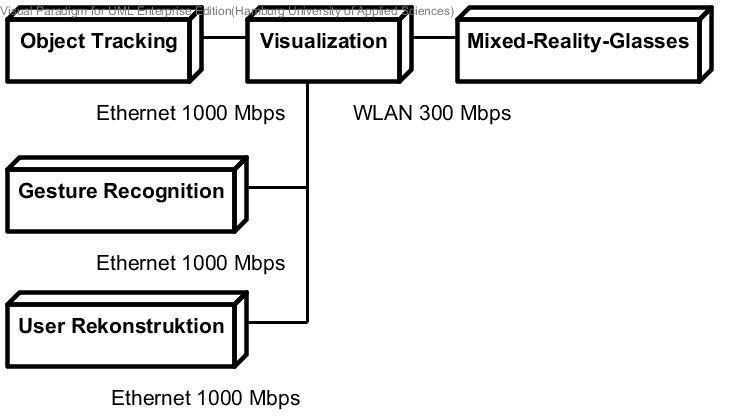
\includegraphics[width=.5\textwidth, keepaspectratio]{img/deployment}
		\caption{Deployment Diagramm des Gesamtsystems}
		\label{fig:bigpicture}
	\end{center}
\end{figure}

In diesem Bericht wird auf die Entwicklung der User Rekonstruktionskomponente eingegangen. Damit der Benutzer in einer dreidimensionalen Umgebung dargestellt werden kann, benötigt man ein 3D Modell welches möglichst seiner aktuellen, äußeren Erscheinung entspricht. Hierfür wird der Benutzer mittels visuellen Sensoren gescannt, um aus den erhaltenen Scandaten ein 3D Oberflächenmodell des Benutzers, zu möglichst interaktiven Frameraten zu berechnen. Damit ein möglichst vollständiges Modell des Benutzers entstehen kann, werden mehrere Sensoren verwendet.

\subsection{Anforderungen}
\begin{enumerate}
	\item Das System unterstützt verschiedene Sensoren über ein gemeinsames Interface.
	\item Das System erfasst simultan 3D Informationen aus $N$ Sensoren.
	\item Das System bietet Methoden um die 3D Informationen in ein gemeinsames Koordinatensystem zu transformieren.
	\item Das System extrahiert Personen aus den 3D Informationen.
	\item Das System bereinigt und fusioniert die Sensordaten und produziert ein geschlossenes 3D-Polygongitter
	\item Die Verarbeitung der Sensordaten soll über definierte, austauschbare Module geschehen, um eine aussagekräftige Auswertung verschiedener Algorithmen zu erlauben.
\end{enumerate}

\subsection{Ausschlüsse und Abgrenzungen}

\begin{enumerate}
	\item In Abgrenzung zu Systemen, welche Motion-Capturing Verfahren zum animieren von virtuellen Avataren verwenden soll dieses System explizit Oberflächenscans von Personen zur 3D Modell Generierung verwenden.
	\item In Abgrenzung zu Systemen, die ein statisches Modell in Echtzeit anfertigen können, soll dieses System die Rekonstruktionszeit für ein 3D Modell so weit reduzieren, dass ein dynamisches Modell in Echtzeit entsteht.
	\item In Abgrenzung zu Phase-Shift Structured-Light Scanning Systemen welche mit sichtbarem Licht sehr hoch aufgelöste Modelle von zum Beispiel Gesichtern erstellen, soll hier zum einen nicht aktiv mit sichtbarem Licht gearbeitet werden sondern vorwiegend im infrarotem Lichtbereich. Weiterhin ist das Ziel nicht eine möglichst hohe Auflösung zu erreichen, sondern ein möglichst performantes und vollständiges 3D Modell von Menschen zu erstellen.
\end{enumerate}

Folgende Ausschlüsse und Abgrenzungen besitzen nur für Projekt 1 Gültigkeit:

\begin{enumerate}
	\item Das System unterstützt zunächst ausschließlich OpenNI2-kompatible Sensoren
	\item Das System ist nicht verteilt und verwendet zunächst eine lokale Visualisierung.
	\item Das System arbeitet zunächst mit einem einzelnen Sensor.
\end{enumerate}

\subsection{Zukünftige Erweiterungen}

\begin{enumerate}
	\item Einbindung von Sensoren über Microsoft Kinect SDK und KinectSDKv2
	\item Parallele Verarbeitung der Sensordaten multipler Sensoren
	\item Streaming des Meshes an eine entfernte Visualisierungskomponente 
\end{enumerate}

\subsection{Glossar}

\begin{enumerate}
	\item Anwendung: Die von der Forschungsgruppe I$^2$E entwickelte Mixed-Reality Anwendung
	\item System: Das User-Reconstruction System
	\item PointCloud: Ein Array von Punkten. Kann organisiert sein, das heißt die Punktwolke kann in eine Matrixstruktur aus Zeilen und Spalten zerlegt werden.
	\item Punkt: Im wesentlichen kartesische 3D Koordinaten. Können durch zusätzliche Datentupel (Farbe, Flächennormale, etc.) angereichert werden.
	\item Sensor: Im Fokus liegen in dieser Arbeit vor allem Tiefenbildkameras, prinzipiell kann dies aber jedes Punktwolken generierende Verfahren darstellen.
	\item Polygonmesh: Im Sinne der 3D Modellierung eine Sammlung von Punkten, Kanten und Flächen, die ein polyhedrales 3D Objekt darstellen.
\end{enumerate}

